% This is a sample file for submissions to the PCJ. To submit, you have to
% prepare a pdf file of all the contents pages of your paper, without the cover
% page: this behavior is triggered by the class option 'mode=plain' below. The
% cover page, including the metadata and the abstract, and the page
% headers/footers will be added upon online publication.
%
% This "author package" does not contain all the files necessary to support
% typesetting of a cover page, if you need to do so please contact the team.

\documentclass[PCJ,Unicode,screen,mode=plain]{cedram}
\usepackage[natbib=true, style=pcj]{biblatex}
\usepackage{lipsum}

% Declare your BibTeX file here (keep the .bib extension):
\addbibresource{references.bib}

% This is to correct wrong references sorting, see sample .bib file.
\providecommand*{\noopsort}[1]{}

%%%%%%%%%%%%%%%%%%%%%%%%%%%%%%%%%%%%%%%%%%%%%%%%%%%%%%%%%%%%%%%%%%%%%%%
%
% Article metadata: these are all commented out here because they only appear on
% the cover page and article headers/footers after publication, and you are not
% asked/expected to generate these elements (there is a separate web interface
% to fill them in during the submission process).
%
% \title[Sample for the template]{Sample for the template, with quite a very long title}
%
% \RDOI{12.3456/pci/rec.fake.123} % DOI of the PCI recommendation
% \setPCI{ecotoxenvchem}
% \PCIcorresp{machin@example.edu}
%
% \author{\firstname{Antoine} \lastname{Lavoisier}\IsEqualContrib}
% \address{Rue sans aplomb, Paris, France}
% \email[A. Lavoisier]{a-lavois@lead-free-univ.edu}
%
% \author{\firstname{Mary} \middlename{P.} \lastname{Curry}\IsEqualContrib}
% \address{Center for spiced radium experiments, United Kingdom}
% \email[M.~P.~Curry]{m.p.curry@radexp.edu.uk}
%
% \author{\firstname{Dick} \lastname{Darlington}}
% \address{Bruce's Bar and Grill, London (near Susan's)}
% \email[D.~Darlington]{dd@example.com}
%
% \author{\firstname{Peter} \lastname{Curry}}
% \address{Center for spiced radium experiments, United Kingdom}
% \email[P.~Curry]{p.curry@radexp.edu.uk}
%
% \keywords{Example, Keyword}
%
% \begin{abstract}
%     \lipsum[1]
% \end{abstract}
%
%%%%%%%%%%%%%%%%%%%%%%%%%%%%%%%%%%%%%%%%%%%%%%%%%%%%%%%%%%%%%%%%%%%%%%%%%%

\begin{document}
% \maketitle
\tableofcontents

\section*{Introduction}

Geometric morphometrics (GM) is a quantitative approach to studying shape in two or three dimensions that has recently been adopted in archaeology (see \autocite[for overviews]{MacLeod2017-yl,Okumura2019-ur,Shott2010-fn}). It has numerous advantages over traditional lithic analyses, particularly because it can overcome the reliance on linear dimensions \autocite[~196-197]{Shott2010-fn}. Lithic artifacts can be assigned to typologies or directly compared without the use of a typology, as will be demonstrated in this paper. There are several approaches within GM that provide similar results through different methods. One of the more traditional approaches is to place landmarks at homologous locations around the object. Landmarks can be augmented with semilandmarks, which are points placed relative to another using a consistent rule---usually equidistant spacing between two points \autocite[2-4]{Okumura2019-ur}. Another common approach is to use elliptical Fourier analysis to compare the outlines of objects. Each method has strengths and weaknesses. A major purpose of this study is to evaluate the effectiveness of these methods for analyzing projectile points in the U.S. Southwest during the late prehistoric period (specifically during the Hohokam Classic Period---AD 1100-1500).

Once the method of analyzing the projectile points has been determined, the next step is to determine how to compare projectile points using the results of the analysis. One approach would be to use an existing regional typology and to assign projectile points to the closest match \autocite[e.g.,]{Kocer2017-au}. Another approach, would be to use cluster analysis to assign projectile points to newly created types \autocites[e.g.,][]{Petrik2018-pd,Matzig2021-id}. The final approach would be to ignore typologies and compare the morphometric distance for each projectile point directly. This is the second primary purpose of this study---to evaluate the effectiveness of these approaches for use in analyzing projectile points from the Southwest United States.

Regional analyses are fundamental parts of archaeology, but there are many challenges to overcome. One of these challenges is harmonizing the different categorization schemes (i.e., ontologies) used throughout the region. Another of these challenges, is determining whether the current categories are useful. The U.S. Southwest has a long history of regional ceramic typologies \autocites[e.g.,][]{Colton1956-zy,gladwin1930a,Hargrave1932-ng,Kidder1915-ae,Martin1940-jg}, but there are still disagreements, challenges, and competing definitions \autocite{Duff1996-au}. Regional analyses in the Southwest, based in large part on pottery, have produced many useful insights \autocites[e.g.,][]{Bernardini2005-ue,Clark2019-bz,Hegmon2016-xw,Mills2013-wq,Peeples2018-ib}. However, one type of material culture that has received little attention---in the Southwest at least---is lithics (i.e., chipped stone). Projectile points are commonly discussed during the archaic period of the Southwest, and they are common topics in many other areas of the North American continent and world where they are found, but they are rarely discussed after the appearance of pottery.

Despite the over-emphasis on pottery in the Southwest, there are some excellent resources on projectile point typologies \autocites[e.g.,][]{Hoffman1997-hb,Justice2002-cf,Loendorf2004-tp,Sliva2006-nq}. However, ad hoc approaches are common, and these cannot easily be extrapolated beyond specific projects. Even using existing resources can make comparisons difficult. How does Tagg's \autocite*[p.111]{Tagg1994-wi} Type 23 compare to Sliva's \autocite*[p.~35]{Sliva2006-nq} Cohonina Side-notched? There is an answer, but often it is easier to come up with a new typology schema than to try to harmonize existing work.

Another challenge that is not unique to projectile points is that interpretations may differ between analysts. Exactly when does a base begin curving enough to be called basal notched? Even the difference between a side-notched and a corner-notched point can, at times, be ambiguous. Not to mention the frustrating situation where a point appears to have one corner-notch and one side-notch. How should one place this point into an existing typology? These are questions that can be handled in different ways that differ from analyst to analyst. Idiosyncrasies and biases are impossible to be rid of entirely, but using approaches such as those described in this paper can reduce them and increase the reproducibility of the process.

By necessity, this paper covers a number of topics. The geographic area is the U.S. Southwest, but the methods and analysis are applicable to any area. The primary purpose was to explore geometric morphometric methods using previously typed specimens from the Southwest and untyped specimens from the Tonto Basin. Another purpose was to analyze the results with and without using typologies. The results demonstrate that, in this particular case, a combined landmark and semilandmark approach is most effective and that useful analyses can be conducted with and without the use of typologies.

\section{Background}

In order to test the effectiveness of geometric morphometric methods, I needed a dataset of well-typed projectile points that could be used as a validation set. I chose to use the typology published by Noel Justice \autocite*{Justice2002-cf} for the simple reason that it is easily accessible and contains numerous illustrations. These illustrations were used as type specimens to compare projectile points from Tonto Basin in central Arizona (Figure 1). These points were excavated in a series of large cultural resource management projects necessitated by work on the Roosevelt Dam. The largest project---the Roosevelt Platform Mound Study---included 129 sites. Most of the sites date between AD 1275 and 1325 with occupation continuing until around AD 1450 \autocite{Rice1998-ku}. In the original analysis, projectile points were classified according to small and large points and then subdivided based on morphological characteristics \autocite[p.727]{Rice1994-rk}. The typology used is an excellent demonstration of the difficulty in conducting projectile point studies in this area, as the typology is idiosyncratic to this specific project, and cannot be easily compared with other datasets. This is not a criticism of the analyst's choice to create a new typology, as no existing typology met the needs of the researchers.

\begin{figure}
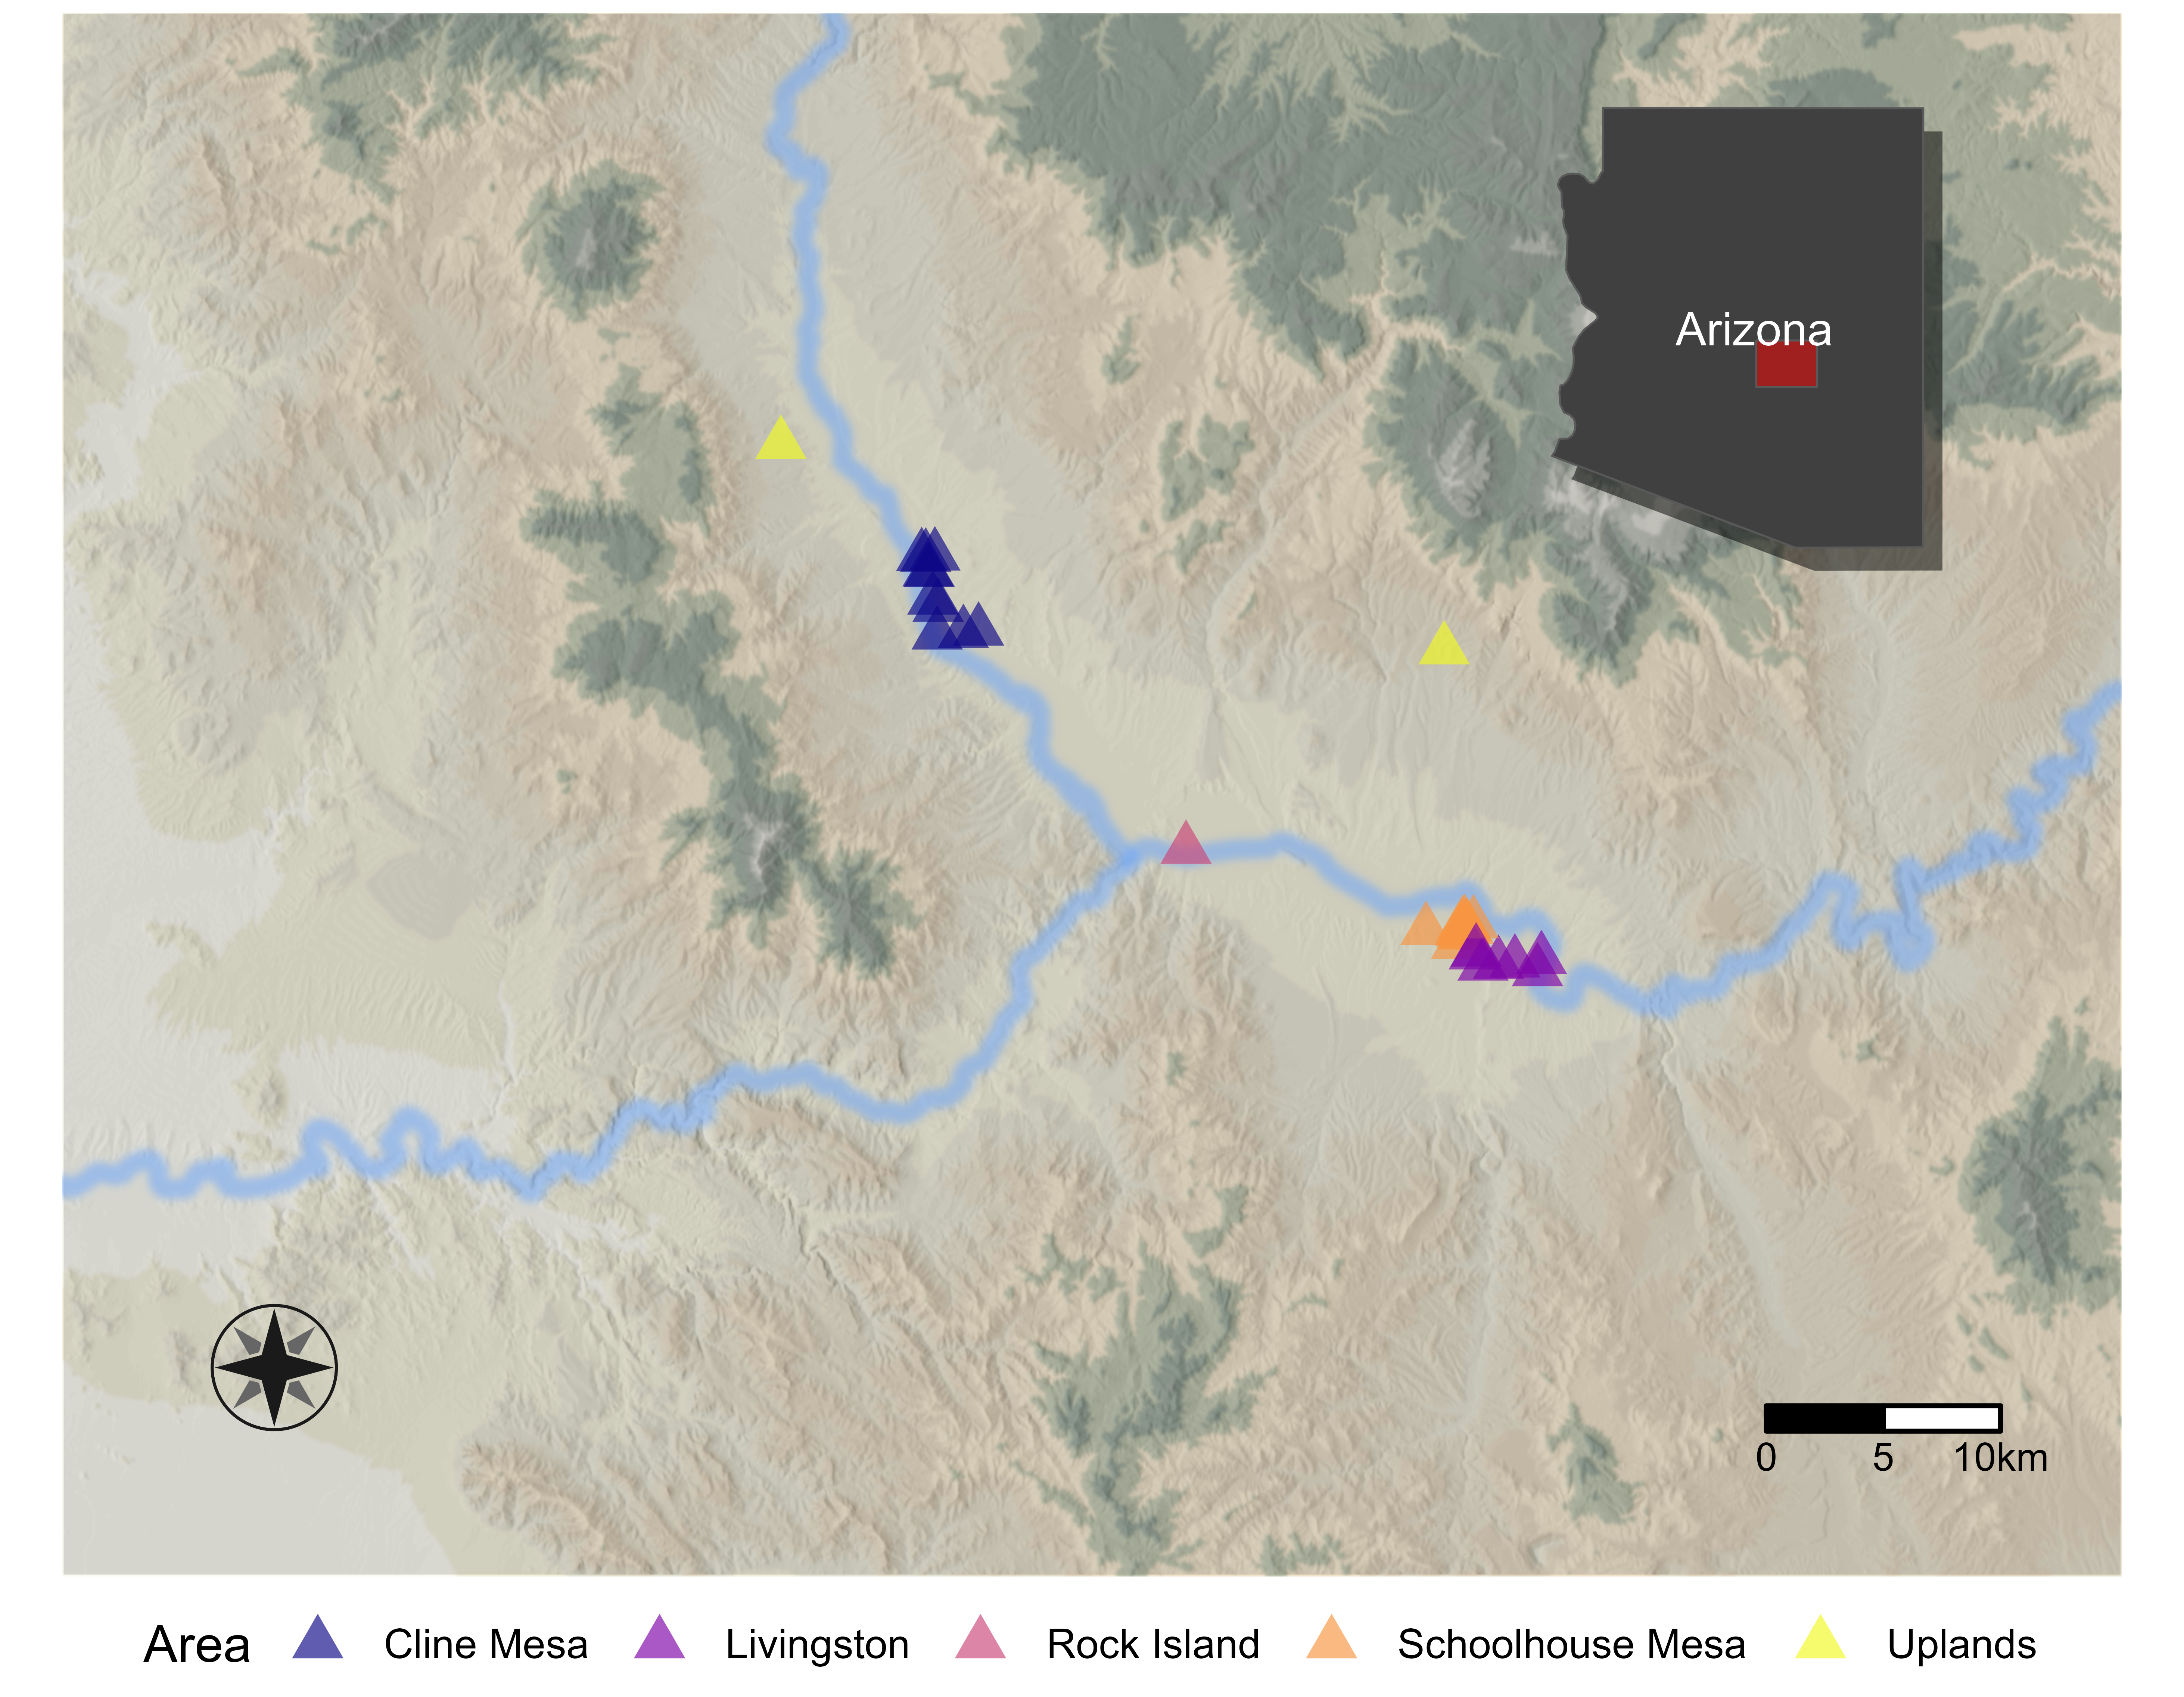
\includegraphics[width=1\linewidth]{TontoBasin} \caption{Location of Tonto Basin in the state of Arizona, United States, along with archaeological sites discussed in this paper grouped by site cluster.}\label{fig:TontoBasinMap}
\end{figure}

This is an exploratory analysis designed to minimize the amount of time spent collecting data and to be as reproducible as possible. There are a number of research steps that are often not addressed in publications. This missing documentation can make reproducing results challenging. I will describe the rational for relevant decisions, but the script used to generate the analysis will be included in an RMarkdown document in the supplemental material (see statement at end of manuscript).

One of the key elements of this study is reproducibility, which necessitates automation. Projectile point analysis often includes assigning a point to a type based on linear metrics---sometimes angular measurements as well, and the presence or absence of various features (e.g., concave base, serrated blades, corner-notches). But often, the analyst is left to visually compare the point to various type specimens to identify the closest match. This method is harder to reproduce and subject to greater human error. Yet, algorithms are only part of the answer, and human judgment and context are still critical to any analysis. The key is to minimize the possibilities for error and maximize the opportunities for reproducibility, which I have tried to do here. Thus, one of the key questions of this research is to determine what input should be left to the analyst and what can be left to automated or standardized procedures.

\subsection{Data Collection}

This study has two sources of data: illustrations of projectile points published by Justice \autocite*{Justice2002-cf} and images of projectile points from collections held at Arizona State University. The datasets include 74 illustrations from Justice's publication and 90 projectile points from Tonto Basin. The 74 illustrations do not include all of Justice's illustrations or types, as many could not be included because there were so few complete, illustrated examples.

It is worthwhile to question how an illustration compares to an image of a physical projectile point obtained from a flatbed scanner. Fortunately, illustrations have been published for some of the projectile points in this study. Figure 2 is a comparison of outlines created from an illustration and scan of the same projectile point. There are subtle differences between the two mediums---the base is slightly more rounded in places than the scan. These differences are detectable in a morphometrics analysis, however, the differences are minor as seen in figure 3. These minor differences would not affect the results of the analyses presented here or most GM analyses. The quality of projectile point illustration can vary, but from this brief comparison there should be no hesitation using illustrations for 2D morphometric analysis.

\begin{figure}
\includegraphics[width=1\linewidth]{pointComparison} \caption{Comparison of projectile point outlines for an illustration and a scan of the same projectile point (Oliver and Simon 1997: Figure 9.3; Specimen 33598)}\label{fig:pointComparison}
\end{figure}

\begin{figure}
\includegraphics[width=1\linewidth]{comparisonPCA} \caption{Principal component (PC) plot comparing the morphometric differences between a sample of 20 random projectile points and the illustration and scan of the same projectile point. The morphospace is also projected. The morphospace computes the projectile point outlines shown in the figure, which represents how shapes vary along each axis. The barchart in top left corner displays proportion each PC contributes to total variance.}\label{fig:comparisonPCA}
\end{figure}

Justice's projectile point illustrations were scanned, and the illustrations were converted into individual, solid black outlines and saved as jpeg files using common image-editing software. The open source statistical software R was used for all analyses \autocite{R_Core_Team2022-wb}. The Momocs package \autocite{Bonhomme2014-gt} has an import function to convert jpeg files into outlines. This is a major advantage over manual outlining processes used in popular GM software, such as tpsDig \autocite{James_Rohlf2015-ui}. These outlines form the the basis of the geometric morphometric analyses conducted here with the exception of the landmark analyses. Landmarking was performed using the tpsDig software. The Tonto Basin projectile point images were created using a flatbed scanner at 1200 DPI \footnote{Many of the images were obtained by the author but some were generously contributed by Joshua Watts---see the results of his study here: \autocite{Watts2013-ub}.}. The images were converted to outlines using the same process as the projectile point illustrations.

\subsection{Projectile Points of the Southwest}

There are a few regional typologies for projectile points in the Southwest: primary examples are Hoffman \autocite*{Hoffman1997-hb}, Justice \autocite*{Justice2002-cf}, Loendorf and Rice \autocite*{Loendorf2004-tp}, and Sliva \autocite*{Sliva2006-nq}. Altogether, these four typologies include 129 projectile point types, although many overlap. In some cases, the authors identify correlates of the types from other typologies. This allows for some harmonization of the different typologies. Many types date to the Archaic period, and thus predate the primary period I am interested in (AD 1100-1500). Not all of the projectile points were ascribed dates by the authors. Justice lists 23 projectile points that overlap with the AD 1100-1500 period (the maximal dates for the Hohokam Classic period). Projectile points have restricted geographical boundaries, although these boundaries correspond to much greater areas than ceramic types typically do \autocite{Buchanan2019-vn}. Figure 4 shows that several projectile point boundaries defined by Justice overlap with the Tonto Basin.

\begin{figure}
\includegraphics[width=1\linewidth]{ProjPointBoundaries} \caption{Location of selected projectile point boundaries defined by Justice (2002) as digitized by Buchanan and colleagues (2019). Darker colors represent greater overlap in the number of projectile point boundaries.}\label{fig:ProjectilePointBoundaries}
\end{figure}

For this study, I digitized 74 projectile point images from Justice's publication representing 8 projectile point types (table 1). Justice placed each projectile point type into a cluster of related points. Figure 5 shows the projectile point outlines by type. The included projectile point types include some Archaic points and types not expected to overlap with the Tonto Basin projectile points. Small numbers of archaic points are often found at later sites. These are likely the result of collecting activities and not indicative of the continued use of these points \autocite[see][ for numerous examples]{Justice2002-cf}. These curated archaic types form useful comparisons, as they should not match non-archaic projectile points. One limitation of this study is that projectile points must be complete, or nearly complete (minor damage to the tip or another part of the point that was judged to not significantly impact the shape of the point was ignored). Thus, not all of the illustrations included in Justice's book could be included in the outline analyses.

\begin{table}

\caption{\label{tab:tblJusticeTypes}Cluster Names, Types, and Number of Samples}
\centering
\begin{tabular}[t]{llr}
\toprule
Cluster & Type & Total\\
\midrule
Chaco & Chaco Corner Notched & 9\\
Chaco & Pueblo Alto Side Notched & 7\\
Cienega & Tularosa Corner Notched & 13\\
Livermore & Guadalupe & 12\\
Pueblo Side Notched & Pueblo Side Notched Concave Base & 9\\
\addlinespace
Pueblo Side Notched & Pueblo Side Notched Straight Base & 7\\
Snaketown & Snaketown Triangular Concave Base & 9\\
Western Triangular & Cottonwood Triangular & 8\\
\bottomrule
\end{tabular}
\end{table}

\begin{figure}
\includegraphics[width=1\linewidth]{JusticePointsTypesFinal} \caption{Outlines of projectile point illustrations taken from Justice (2002). Note that the projectile points are not scaled.}\label{fig:JusticePointsTypesFinal}
\end{figure}

\subsection{Tonto Basin Projectile Points}

The sample of Tonto Basin points used in this study come from the Roosevelt Platform Mound Study. They come from 18 different sites that were grouped into five clusters in the original reports \autocite[see][ for an overview]{Rice1998-ku}. Figure 1 shows the sites used in this study grouped by site cluster. The majority of these sites were occupied during the Roosevelt phase (AD 1275-1325) and early portion of the Gila phase (AD 1325-1450). The sites consist primarily of compounds, room blocks, and platform mounds.

The projectile points exhibit a variety of forms (see figure 6). Rice \autocite*{Rice1994-rk} classified Tonto Basin points into small and large complexes (likely equivalent to dart and arrow points), and further classified small points into the longer Salado series and the shorter Tonto series. These series were further subdivided using a custom classification scheme based on blade, tang, and base shape, as well as notch style. This is a logical way to classify the points, but it does not easily lend itself to regional comparisons, as other points were not classified in the same way. Nearly all of the points in the original sample consisted of side-notched or triangular points. Because the results of the analysis discussed below indicated that analyzing the projectile points by shape was the most logical choice, only the triangular and side-notched points were used in this study.

\begin{figure}
\includegraphics[width=1\linewidth]{TontoPointsFinal} \caption{Outlines of projectile points from sites in the Tonto Basin. Note that the projectile points are not scaled.}\label{fig:TontoPointsFinal}
\end{figure}

\section{Methods}

\subsection{Geometric Morphometrics}

I used two GM methods in this analysis: elliptical Fourier analysis (EFA) and full generalized Procrustes alignment (GPA). Something to keep in mind is that GM methods analyze the form of the object separated from size, position, and orientation. Real-world measurements such as length and width are not explicitly included in these methods, although relative dimensions, such as length to width ratio are captured in the overall form of the object. Measurements such as length and weight can be included in various analyses but are not included here. The purpose of this study is to determine whether GM methods alone are sufficient to discriminate between types of projectile points and how they can best be used in the context of the U.S. Southwest.

EFA was developed by Kuhl and Giardina \autocite*{Kuhl1982-kd} as a quantitative means for describing a closed outline. There are a handful of papers that use EFA for lithic studies in archaeology \autocites[e.g.,][]{Cardillo2010-ys,Fox2015-ox,Gingerich2014-cb,Hoggard2019-yw,Iovita2011-nz,Iovita2011-zp,Matzig2021-id}. The mathematics behind the method are complex to describe, which is one reason the method has not been adopted as quickly as it should be \autocite[see][]{Caple2017-mk}. Caple and colleagues \autocite*{Caple2017-mk} provide an excellent description of EFA for non-mathematicians, and the reader is referred to their treatise for more details. For my purposes, it is enough to know that EFA analysis requires a closed outline and a number of harmonics. The harmonics can be thought of as ellipses in a time series used to describe the shape of the object. EFA creates a series of coefficients---four for each harmonic (A,B,C,D)---which can be used in multivariate statistics. Most commonly, principal components analysis (PCA) is used to transform the EFA values. The PCA results can then be used in distance-based methods such as clustering or even network analysis. Three harmonics can be used to create an oval shape, and 12 harmonics is sufficient for a complex projectile point outline. The number of harmonics necessary to capture the outline to a certain accuracy can be computed by first calculating the harmonic power using the formula: \[ HarmonicPower_n = \frac{A^2_n+B^2_n+C^2_n+D^2_n}{2} \] where n is the number of harmonics and A, B, C, and D are the coefficients generated from the EFA. The harmonic power is first calculated for a maximum number of harmonics and then the desired proportion (e.g., 99\%) of the harmonic power can be used as a baseline to determine which number of harmonics has at least that much harmonic power.

Generalized Procrustes Analysis, or GPA, is primarily a way to align, scale, and rotate landmarks \autocite{Gower1975-uv}. Instead of outlines like EFA, GPA requires landmarks located on homologous locations for each object \autocite{Rohlf1990-mp}. As an alternative to landmarks, semilandmarks can be placed at equidistant locations around the object. Landmarks and semilandmark approaches can be combined. There is substantial discussion on the validity of certain types of landmarks and the use of semilandmarks as landmarks \autocites[e.g.,][]{De_Groote2011-mh,MacLeod2017-yl,Okumura2019-ur,Shott2010-fn}. One disadvantage of traditional landmark analysis, compared to EFA, is that the analyst must be more involved in the selection of the number and placement of landmarks. Once the landmarks, or semilandmarks are placed on the objects, they are iteratively modified to achieve the best possible alignment between shapes without changing the relative positions between landmarks. This modification is done using the GPA procedure. As with EFA, the next step is usually to perform a PCA analysis. Landmark analysis using GPA is more common, so far, in archaeological analysis of stone tools than EFA \autocites[e.g.,][]{Archer2018-zi,Bischoff2020-zn,Buchanan2015-dx,Charlin2018-yg,Fisher2018-jq,Gingerich2014-cb,Herzlinger2017-ce,Lycett2010-od,Riede2019-gb,Selden2020-ni,Shott2010-fn,Smith2015-qk,Thulman2012-fo}.

The project was initially designed to compare the EFA results with a semilandmark analysis using the full outline of the projectile point. The projectile point outline consists of a series of coordinates describing the outline. Semilandmarks can be obtained by sampling the outlines to create an equal number of coordinates, which are then treated as semilandmarks. Both approaches yielded similar results, but neither achieved satisfactory accuracy. The research design was then modified to include a more traditional landmark analysis to determine whether it would improve upon the initial design.

There are some disadvantages to using landmarks, which is why the EFA/semilandmark approach was initially favored. The principal disadvantages to using landmarks are reproducibility and accuracy. Landmarks are more subjective in many ways than the semilandmarks or EFA \autocite[see][205]{Shott2010-fn}. The analyst must decide how many points to place, what topological points should be used as landmarks, and how many landmarks should be used. The placement of landmarks can vary between analysts and can be affected by the instruments or software used to collect or create the landmarks. Another major concern is the loss of detail from not considering the entire outline. Serrated projectile points and points with more than one notch (this occurs more often than one might expect in Southwestern projectile points) are difficult to capture without including many landmarks, which are only applicable in a minority of situations. Secondary to these points, but still a concern, is that placing landmarks can be a more time-consuming process, as it is not as easily subject to automation as semilandmarks or EFA \autocite[although see][ for one of several examples of automation]{Palaniswamy2010-sl}.

Despite the disadvantages, landmarks are widely used for good reasons. I see two main advantages to landmark analysis in the context of projectile point analysis. The first is that the analyst can use their prior experience to determine what topological locations on the projectile point are most useful for discriminating between types. Decades of research on projectile points has refined many typologies into useful tools, despite their limitations. This knowledge can be applied to choosing appropriate landmarks. The second advantage is that outline analysis requires complete projectile points, whereas landmark analysis can use damaged points. If chunks of the projectile are missing then the outline is not usable. Possibly, the missing portion could be estimated and filled in, but that process is more error prone than estimating missing landmarks. Landmarks can be placed on reconstructed projectile point illustrations or missing landmarks can be estimated mathematically \autocite{Gunz2009-yb}. Most projectile points suffer from some type of damage and some of the projectile points I classified as ``complete'' suffer from minor damage to the tip of the point or elsewhere. The use of damaged points can greatly increase the available sample size for studies, which is often a major limitation in projectile point studies.

Landmark configurations can vary significantly, depending on what the analysis is designed to measure and on the point type. Most projectile point landmark analyses incorporate both landmarks and semilandmarks. The difference being that landmarks are placed on homologous points (notches, corners, etc.) and semilandmarks are placed equidistantly along a curve or line. Most of the area of a projectile point is usually in the blade---the portion above the notches. The base of the point, the portion below the notches, is also the hafting element. For projectile point typologies, the base of the point usually contains the most important elements for determining the type---notching style and basal shape being the two major elements. Thus, if most of the landmarks or semilandmarks are on the blade margins then the base of the point is not getting as much coverage. It is more than just tradition that the base gets the most attention. Hafting a point is an important technological choice, more so than how long the point is. Furthermore, projectile points can be resharpened. Resharpening the blade margins can modify the shape of the blade and change its appearance. While it is possible to modify the base of the point and even convert a side-notched point into a corner-notched point and vice-versa, it is unlikely that this happened regularly with the small arrowpoints used in this study \autocite{Loendorf2019-df}. Because it is necessary to incorporate different landmarking procedures for each projectile point shape, I separated the projectile points into three classes: side-notched, corner-notched, and triangular. For this study, I combined stemmed points into the corner-notched category.

Because of the vagaries of placing landmarks, I used two configurations in this study. In the first configuration, the full outline was used. In the second configuration, I used what I term the ``corner'' of the projectile point. Figure 7 shows the first landmark configurations. For simplicity, I will refer to both landmarks and semilandmarks in the following discussion as landmarks. The landmark configuration was designed to place fewer landmarks along the blade margins and more landmarks along the notches and the base. Separate curves were placed between the tip of the point and the notches and the notches and the base (or the tip and the base for triangular projectile points), and landmarks were placed at equidistant locations along the curves. The second configuration is much sparser (figure 8). The landmarks were placed only on the right side of the point. For the side-notched and corner-notched projectile points, landmarking started from the top of the notch, moved to the middle of the notch and then the bottom portion of the notch. For corner-notched points, this last landmark marked the right corner of the point, but for side-notched points an additional landmark was needed to mark the base of the point. The final landmark was placed at the center of the basal margin. Triangular points differed by placing the first landmark in the center of the blade margin. The first approach contains between 30 and 42 landmarks that cover the entire point outline, whereas the second ranges from 3 to 5 landmarks that cover only a portion of the projectile point. These extremes were chosen to provide significant contrast between approaches.

\begin{figure}
\includegraphics[width=1\linewidth]{curveComparison} \caption{Comparison of the full outline landmarks for corner-notched, side-notched and triangular shaped projectile points from Justice's (2002) projectile point illustrations. Red dots indicate the mean location for each of the landmarks.}\label{fig:curvesStack}
\end{figure}

\begin{figure}
\includegraphics[width=1\linewidth]{cornerComparison} \caption{Comparison of the projectile point corner's landmarks for corner-notched, side-notched and triangular shaped points from Justice's (2002) projectile point illustrations. Red dots indicate the mean location for each of the landmarks.}\label{fig:cornerComparison}
\end{figure}

\section{Results}

\subsection{Justice Projectile Points}

The first step in the analysis was to determine how well projectile points typed by Justice could be correctly assigned using GM methods. Linear discriminant analysis (LDA) was used to type the projectile points using the GM results. A general target of 0.85 was arbitrarily chosen as a minimum target for acceptable results---meaning that 85\% of the projectile points were classified correctly. As mentioned previously, Justice placed each projectile point type into a cluster. Presumably, projectile point types in the same cluster should be more closely related than they are to projectile point types in other clusters. This gives another level of comparison that was used in addition to the types.

The original intent was to compare EFA versus semilandmarks placed at equidistant locations around the outline. However, these results were unsatisfactory, and a more traditional landmark analysis was also completed. Because the number and placement of landmarks has a significant impact on the outcome of the study, two different landmark configurations were used. Tables 2, 3, and 4 show the LDA results by type, cluster, and by shape---the column and row means are also included. These tables will be referred to in the sections that follow.

Part of the reason the results were unsatisfactory for the EFA and semilandmarks was that the LDA analysis had trouble discriminating between notched and unnotched projectile points and between side-notched and corner-notched points. These are some of the most basic distinctions that are made when analyzing projectile points. While it would be convenient if the analysis did not require an additional step, it is not difficult to separate the projectile points into these basic shapes prior to the GM analysis. Table 2 shows the accuracy of EFA and semilandmark analysis for identifying each type of shape. The landmark analysis was not compared as each shape used a different landmark configuration. The primary challenge was identifying side-notched from triangular points.

\begin{table}

\caption{\label{tab:LDAResultsShape}Linear Discriminant Analysis Results for Projectile Point Shapes}
\centering
\begin{tabular}[t]{lrrr}
\toprule
Shape & EFA & semiLdk & Mean\\
\midrule
Corner-notched & 0.88 & 0.91 & 0.90\\
Side-notched & 0.65 & 0.74 & 0.70\\
Triangular & 0.76 & 0.59 & 0.68\\
Mean & 0.76 & 0.75 & \\
\bottomrule
\end{tabular}
\end{table}

\begin{table}

\caption{\label{tab:LDAResultsType}Linear Discriminant Analysis Results for Projectile Point Types}
\centering
\begin{tabular}[t]{lrrrrr}
\toprule
Type & EFA & semiLdk & Ldk & Ldk-corner & Mean\\
\midrule
Chaco Corner Notched & 0.56 & 0.89 & 0.85 & 0.85 & 0.79\\
Cottonwood Triangular & 0.38 & 0.38 & 1.00 & 0.75 & 0.63\\
Guadalupe & 0.75 & 0.83 & 0.93 & 0.93 & 0.86\\
Pueblo Alto Side Notched & 0.86 & 0.71 & 1.00 & 1.00 & 0.89\\
Pueblo Side Notched Concave Base & 0.44 & 0.78 & 0.73 & 0.73 & 0.67\\
\addlinespace
Pueblo Side Notched Straight Base & 0.57 & 0.57 & 0.43 & 0.71 & 0.57\\
Snaketown Triangular Concave Base & 0.78 & 0.89 & 0.78 & 0.89 & 0.84\\
Tularosa Corner Notched & 0.77 & 0.69 & 0.60 & 0.80 & 0.72\\
Mean & 0.64 & 0.72 & 0.79 & 0.83 & \\
\bottomrule
\end{tabular}
\end{table}

\begin{table}

\caption{\label{tab:LDAResultsCluster}Linear Discriminant Analysis Results for Projectile Point Clusters}
\centering
\begin{tabular}[t]{lrrrrr}
\toprule
Cluster & EFA & semiLdk & Ldk & Ldk-corner & Mean\\
\midrule
Chaco & 0.81 & 0.88 & 0.92 & 0.92 & 0.88\\
Cienega & 0.69 & 0.69 & 0.60 & 0.80 & 0.70\\
Livermore & 0.83 & 0.75 & 0.93 & 0.93 & 0.86\\
Pueblo Side Notched & 0.75 & 0.56 & 0.89 & 1.00 & 0.80\\
Snaketown & 0.78 & 0.89 & 0.78 & 0.89 & 0.84\\
\addlinespace
Western Triangular & 0.38 & 0.50 & 1.00 & 0.75 & 0.66\\
Mean & 0.71 & 0.71 & 0.85 & 0.88 & \\
\bottomrule
\end{tabular}
\end{table}

\subsubsection{Elliptical Fourier Analysis}

The EFA analysis was conducted using the Momocs packages \autocite{Bonhomme2014-gt} in R \autocite{R_Core_Team2022-wb}. The first step was to calculate the number of harmonics to use. In this case 12 harmonics described 99\% of the variation in the projectile point outlines. Next, the EFA function was used on each projectile point, and then a PCA was used to reduce the dimensionality of the data. Figure 9 shows the results of the PCA analysis. A useful feature of PCA plots using these data is that the morphospace can be plotted with the PCA results. The morphospace shows how the shapes vary along each axis of the PCA. In this case, PC1 (the first principal component) varies between short, wide projectile points and long, narrow points. Some of shapes on the top and bottom left have inverted into impossible shapes, but note that no projectile points fall into these areas. PC2 varies primarily from stemmed points to side-notched projectile points.

\begin{figure}
\includegraphics[width=1\linewidth]{JusticeEFAPCA} \caption{Principal components (PC) plot showing projectile points from Justice (2002) and the morphospace based on an elliptical Fourier analysis. The projectile points are labeled by the cluster assigned by Justice. The barchart in bottom right corner displays proportion each PC contributes to total variance.}\label{fig:JusticeEFAPCA}
\end{figure}

The first objective for the analysis of the Justice projectile points is to determine how well the different point types can be discriminated. Meaning, how well can GM methods classify these projectile points into their original categories. The LDA results were far from the target goal of 0.85 for most projectile point types, and only one type (Pueblo Alto Side Notched---0.86) met the target (see EFA results in Table 3). The LDA results were better when the projectile point types were grouped into clusters, as shown in Table 4; however, none of the clusters met the target of 0.85. Even more disconcerting were the results shown in Table 2, as only the corner-notched projectile points were discriminated with an accuracy greater than the target.

The differences in classification accuracy between corner-notched, side-notched, and triangular projectile points can perhaps best be explained by examining the mean shapes of each point, as generated through EFA. Figure 10 shows the mean shapes for the selected projectile point types. These are the mathematically average shapes when all of the projectile points in the type are combined. This has a tendency to average out the notches for the side-notched points, as the placement of these notches vary in height. Pueblo Alto Side Notched points appear to be an exception to the side-notched problem, as they have the highest classification accuracy. Corner notched and stemmed points must, by definition, always have their notches or stems in the same location, even though the shape of the notches and stems still varies. This explains why it is easier to discriminate them from other point types. As for the side-notched and triangular points, sometimes the notches are subtle and the notches are only a small part of the whole form, which is clearly not a strong enough element to separate triangular and side-notched points consistently.

\begin{figure}
\includegraphics[width=1\linewidth]{meanShapesEFA} \caption{Mean shapes by projectile point type using elliptical Fourier analysis.}\label{fig:meanShapes}
\end{figure}

\subsubsection{Semilandmarks}

Analyzing projectile points using semilandmarks is comparable to the EFA analysis. The major analytical choice is how many landmarks to use. Each projectile point is represented by a varied number of coordinates that represent its outline. The number of points must be standardized so that each projectile point has an identical number of coordinates, which is done using the Momocs package. The choice of how many points to use does affect the GM analysis. To solve this problem, I tried different numbers of semilandmarks varying from 10 to 100. More than 100 points appears to no longer have a substantial effect on the results. Each projectile point was sampled multiple times and then all of the points were classified using LDA according to the same procedures used for the EFA analysis. The results of this test ranged from 65\% accuracy (10 points) to 73\% accuracy (30 points---the number used for the final analysis) with points higher than 30 consistently measuring in at 64\% accuracy.

The PCA components had similar dimensions of variation as the EFA analysis (see figure 11). The major improvement in accuracy (the `semiLdk' column of Tables 2-4) is perhaps due to the better alignment generated by the GPA procedure, but that is only speculation.

\begin{figure}
\includegraphics[width=1\linewidth]{JusticeSLDKPCA} \caption{Principal Components (PC) plots showing projectile points from Justice (2002) and the morphospace based on a semilandmark generalized procrustes alignment. The projectile points are labeled by the cluster assigned by Justice. The barchart in bottom right corner displays proportion each PC contributes to total variance.}\label{fig:JusticeSLDKPCA}
\end{figure}

Regardless of the reason, a jump from 64\% classification to 72\% between the EFA and semilandmark analysis is a substantial improvement. It does not reach the target of greater than 85\% classification accuracy, but it is a step in the right direction. The mean shapes are nearly identical to the EFA analysis, which indicates that this method suffers from the same problems with side-notched and triangular projectile points, but it does a somewhat better job differentiating corner-notched and side-notched points. Curiously, it does a worse job differentiating triangular points. The side-notches are the likely culprit.

\subsubsection{Landmarks}

Neither the semilandmarks nor EFA adequately distinguished between point types or between point shapes. Identifying notches was particularly troublesome. A solution to this problem was to use landmarks and explicitly identify the notches or lack of notches. No comparison was made between projectile point shapes (i.e., triangular versus side-notched) using landmark analysis, as initial experiments determined that it was best to use different landmark procedures for the different shapes. Perhaps machine learning may solve this problem \autocites[see][]{Castillo_Flores2019-cs,MacLeod2018-aj,Nash2016-mc}. Triangular projectile points require a different approach than side-notched points, and even side-notched and corner-notched/stemmed points require different procedures.

The LDA results for the first landmark configuration (Ldk in Tables 3-4) are much better than EFA and better than the semilandmark analysis, but still not as accurate as desired. The biggest underperformer by far was Pueblo Side Notched Straight Base at 0.43. All of the previous analyses struggled to capture basal shape distinctions, but this analysis struggled more so, as the base is a critical component of this type. What is particularly notable is that Cottonwood Triangular projectile points were classified perfectly whereas they were previously the worst performing type in the EFA and semilandmark analyses. As Table 4 shows, the cluster assignments performed well. If Cienega points were not so problematic, then the results would be excellent.

The final analysis used the second landmark configuration---the projectile point corners. These results proved superior to the first landmark configuration and are almost 20\% higher in accuracy than the EFA results on average. The lowest type for accuracy was again Pueblo Side Notched Straight Base, but it improved from the first landmark configuration to 0.71 from 0.43. The accuracy results were more consistent and accurate. With some additional experimentation on landmark placement, this configuration could likely achieve better results and meet the targeted 0.85 accuracy.

Not only did landmark analysis provide superior accuracy, but it will also make it easier to use larger sample sizes. Presumably, notching style is an important attribute that should be captured in the analysis. If EFA or the semilandmark analysis as conducted here fails to sufficiently emphasize the notches, then these methods are insufficient for classifying projectile points. While landmark analysis is more time-consuming, the use of the second configuration does reduce the burden of landmarking.

\subsection{Tonto Basin Projectile Points}

The initial intent was to classify the Tonto Basin projectile points using the analysis of the Justice projectile points; however, the limited sample size limits the validity of the exercise. The analysis was not futile though, as the second landmark configuration using the corners of the projectile points proved the most effective. I therefore used the same landmark configuration to analyze the projectile points from Tonto Basin. The results of the GPA and PCA analysis were used in a hierarchical cluster analysis using Ward's method \autocite[see][]{Murtagh2014-mb}. Figure 12 is a network graph showing the results. This graph shows the assigned projectile point types from the cluster analysis with connections from every Tonto Basin site where that projectile point was found to the assigned type. Several sites in Tonto Basin only had one or two types of projectile points (low sample sizes were again problematic), but some of the larger, well-excavated sites shared all or most of the projectile point types. It is beyond the purpose of this study to explore the patterns in this data, but the methods clearly provide useful data for exploratory analysis.

\begin{figure}
\includegraphics[width=1\linewidth]{TontoClusterNetwork} \caption{Bipartite network graph displaying assigned projectile point clusters for side-notched and triangular projectile points in Tonto Basin and Tonto Basin sites. The circles represent cluster designations by shape (e.g., side = side-notched and tri = triangular). The squares represent sites. The links between squares and circles show which point clusters are found at which sites.}\label{fig:TontoClusterNetwork}
\end{figure}

The final question I wished to address in this study was whether it was necessary to use a typology in a GM analysis of projectile points. There are many ways to answer this question, but in short, the answer is no. That does not mean typologies are not useful, but they can mask important variation. The following is one way to approach analyzing projectile points without using a typology.

Because the results of the GM analyses can be projected into multidimensional space, the distance between these values is meaningful and can be directly compared. One way to flatten multidimensional space into two dimensions is to calculate the Euclidean distance between each point and display the results as a network graph, as in figures 13 and 14. This way each point can be compared directly without grouping the projectile points into types. The results are messier than neatly fitting each point into a single type, but subtle variation in morphology is easier to visualize this way. The results should only be interpreted as a visual aid. The closer the projectile points are to each other, the more similar they are in shape, keeping in mind that only the corners of the projectile points (from the notches down for the side-notched points) were used in this analysis. Many of the points clustered closely together, indicating a common shape across the sites. The side-notched points have a particularly large cluster of typical Hohokam side-notched points. Yet there are also a large number of projectile points that do not closely match the other points, which indicates that there is also a lot of variation. This variation may represent idiosyncracies, exchange, migration, novice knappers, or a different intention for the point. Regardless of the purpose, the GM analysis better captures the ``otherness'' of a projectile point than classifying a point as other/unknown or worse, forcing it into a category it does not belong in.

\begin{figure}
\includegraphics[width=1\linewidth]{TontoSideDistanceNetwork} \caption{Network graph displaying side-notched projectile points from Tonto Basin as nodes with ties showing the morphometric distance (euclidean distance in Principal Component space) between projectile points. Darker colors represent stronger ties. Note that only the strongest 10\% of ties are shown.}\label{fig:TontoSideDistanceNetwork}
\end{figure}

\begin{figure}
\includegraphics[width=1\linewidth]{TontoTriangularDistanceNetwork} \caption{Network graph displaying triangular projectile points from Tonto Basin as nodes with ties showing the morphometric distance (euclidean distance in Principal Component space) between projectile points. Darker colors represent stronger ties. Note that only the strongest 10\% of ties are shown.}\label{fig:TontoTriangularDistanceNetwork}
\end{figure}

The clustering analysis provided several different projectile point types and provided an overview of what sites shared similar projectile points. This type of analysis can be combined with architectural or other data to look for correlations or patterns that provide insights into the behavior of the people who made and used these projectiles. Yet the analyst must take care to ensure the clustering groups are appropriately sized and the results make sense. One way to view the data more closely is to look at a distance network graph to view the variation in morphometric shape. This way typological distinctions will not mask the variation.

\section{Conclusion}

The purpose of this paper was to evaluate geometric morphometric methods for analyzing projectile points in the Southweset U.S. These analyses provided significant variation in their results, yet they also demonstrated positive results. While EFA underperformed all of the other analyses, a different dataset may favor this analysis. Some of the types performed better for EFA than other types, which suggests that EFA may be the optimal choice for some datasets. Indeed a recent case study found that EFA performed comparable to or better than landmark analysis in several case studies \autocite{Matzig2021-id}. A clear result from this exploratory analysis is that GM analysis is not a one-size-fits-all approach. Better results were obtained from a full outline approach using semilandmarks, which raises interesting theoretical questions I am unable to address here but would be worthwhile to pursue further. More traditional landmark approaches performed better, likely because the outline approaches failed to identify side-notches consistently. In this case, a landmark/semilandmark method using the corner of the projectile point---from the base to the middle of the basal margin or from the middle of the blade if the point is triangular---proved to be the most useful method. The main advantage of this method was that it provided the most accurate reproduction of Justice's original classification of the projectile points. Another advantage is that broken points are easier to use with this method. If one half of the point is missing, either the top or the lateral margin, it does not affect the analysis. This increases the number of points available for analysis tremendously compared to only using whole points. The final advantage, though minor, is that the landmarking analysis is simple and only requires three to five landmarks.

I mentioned how difficult it is to conduct regional analyses with projectile points in the U.S. Southwest. The main difficulty is harmonizing existing typologies and then fitting new projectile points into this typology. While the sample size available for this study was too small to attempt classifying the Tonto Basin points according to Justice's typology, it would be possible to do so with these methods given enough data. However, this paper also demonstrated that it is possible to type projectile points using common clustering methods which may better capture the variation in projectile point morphology than previously used types. Furthermore, it is possible to analyze projectile points without resorting to types. The distances between projectile point morphologies can be computed and compared directly. These distances could even be aggregated and summarized regionally. The main challenge for the regional analysis is obtaining the projectile point outlines or landmarks. Once these are obtained, thousands of points can be analyzed and assigned to clusters relatively quickly.

Compared to a traditional analysis of linear metrics and weights, a GM analysis can capture much more information and provide more informative ways to analyze and visualize the data. The visualization capabilities of GM is one of its greatest strengths, as it allows the analyst to see the data they are working with, visually validate their results, and share their findings in visually compelling ways. Additionally, this analysis is more reproducible and adaptable than traditional lithic analyses. While the analyst still has a lot of control over a GM analysis, the results should be less biased than analyses based on visual type comparisons.

\section*{Acknowledgements}

Special thanks to Zac Selden, Michael Shott, Bernard Means, and Loren Davis for teaching a geometric morphometric workshop that was my first major introduction to these methods. Joshua Watts, Matthew Peeples, Melissa Powell, Christopher Caseldine, and several volunteers assisted with this research.

\section*{Data, scripts, and supplementary information availability}

All relevant data and scripts are available at the following \href{https://osf.io/zge9q/}{DOI 10.17605/OSF.IO/ZGE9Q} and on GitHub at \url{https://github.com/bischrob/TontoBasinPoints}. The R code used in the analysis is included in the manuscript.Rmd file used to create this manuscript, although some lines have been commented out to improve efficiency.

\section*{Conflicts of interest disclosure}

The author declares that they comply with the PCI rule of having no financial conflicts of interest in relation to the content of the article.

\nocite{Oliver1997-lk}

\printbibliography[notcategory=ignore]              %%% add text proper

\end{document}
